\documentclass{beamer}
\usepackage[T1]{fontenc}
\usepackage[utf8]{inputenc}
\usepackage{lmodern}

\usepackage[frenchb]{babel}
\frenchbsetup{StandardLists=true}

\usepackage{color}
\usepackage{graphicx}
\usepackage{amsmath}
\usepackage[framemethod=tikz]{mdframed}


\usetheme{Boadilla}
\usecolortheme{seagull}
\usefonttheme{structurebold}


% Définition du répertoire contenant les images
\graphicspath{{../IMAGE/}}

\title{Mobilité quotidienne et TIC}
\author{Hadrien \textbf{Commenges}, Julie \textbf{Fen-Chong}}
\date{}

\begin{document}


% FRAME
\begin{frame}


\includegraphics[width=12cm]{Logos.pdf}

\vspace*{1cm}

\titlepage

\begin{center}
{\small
Université de Bourgogne

\vspace*{0.1cm}

Master Transports Mobilité Environnement Climat

\vspace*{0.1cm}

3-4 novembre 2014}

\end{center}

\end{frame}


% FRAME
\begin{frame}{Cadrage du sujet}

\begin{figure}
  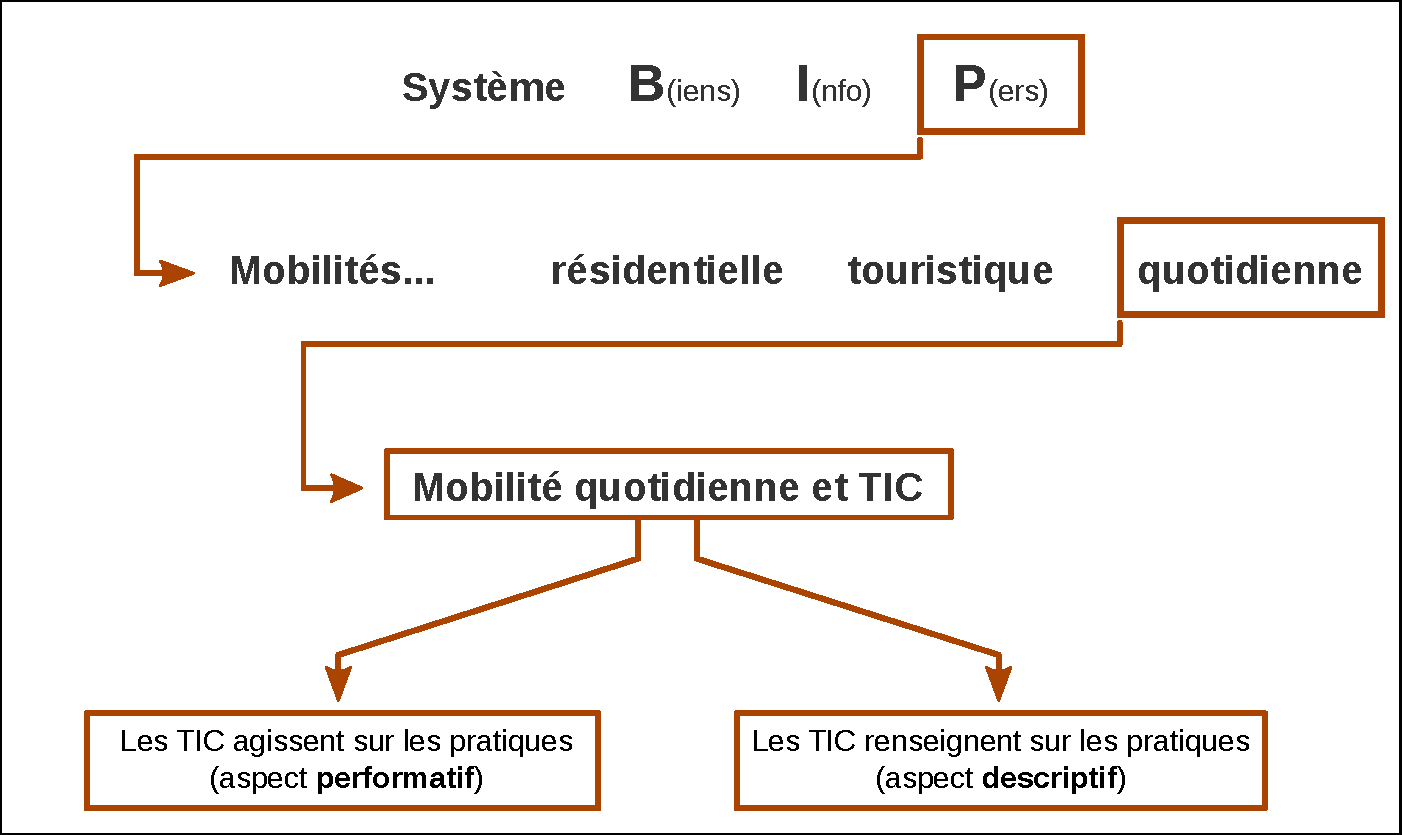
\includegraphics[width=11cm]{Cadrage.pdf}
\end{figure}

\end{frame}


% FRAME
\begin{frame}{Aspects performatifs des TIC}

\emph{"The telephone is an irresistible intruder in time and space"} ~\\
(Marshall McLuhan, 1964)

\footnotesize
\begin{itemize}
  \item Efficacité sociale de la technique
  \item Déterminisme technologique
  \item Vision pessimiste: désurbanisation, fin de la centralité urbaine
  \item Vision optimiste: substitution du transport, rééquilibrage des territoires
  \item Mobilité - TIC : substitution ou complémentarité (voire induction)
\end{itemize}

\normalsize

\begin{figure}
  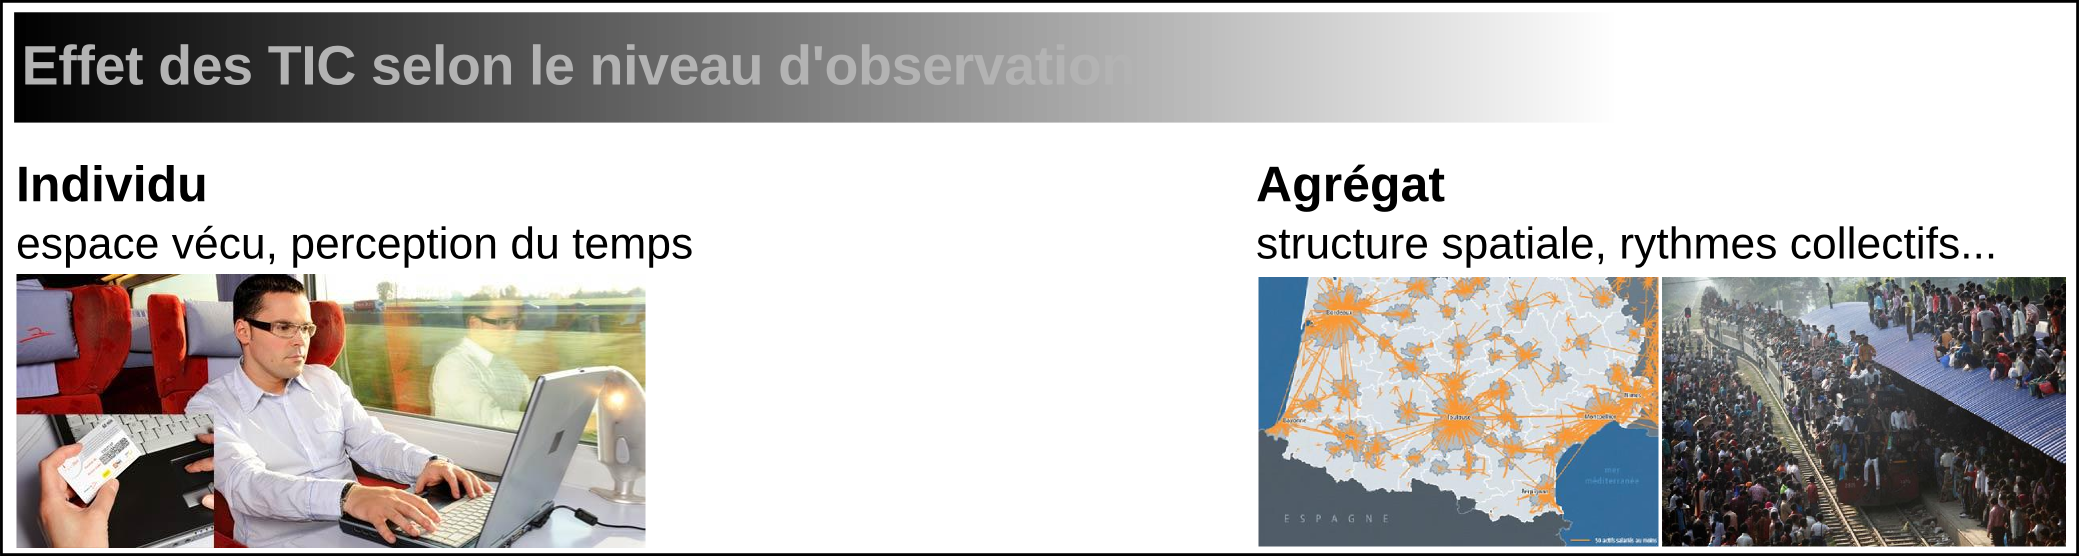
\includegraphics[width=12cm]{IndivAgreg.png}
\end{figure}

\end{frame}


% FRAME
\begin{frame}{Aspects descriptif des TIC}

\begin{figure}
  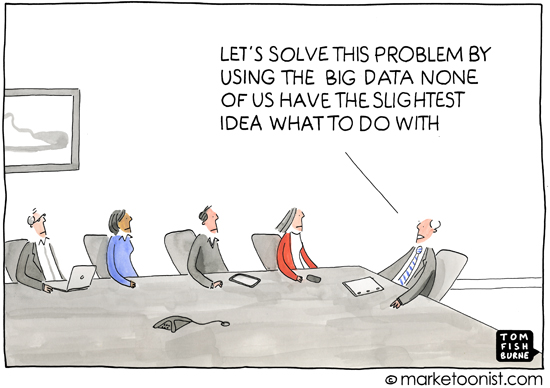
\includegraphics[width=10cm]{bigdata.jpg}
\end{figure}

\end{frame}


% FRAME
\begin{frame}{Appréhender la mobilité quotidienne}

\begin{itemize}
  \item \textbf{Naissance de l'objet \textit{mobilité quotidienne}:} ingeniérie du trafic et sociologie urbaine
  \item \textbf{Constitution des instruments:} ingeniérie du traffic et socio-économie des transports
\end{itemize}

\begin{figure}
  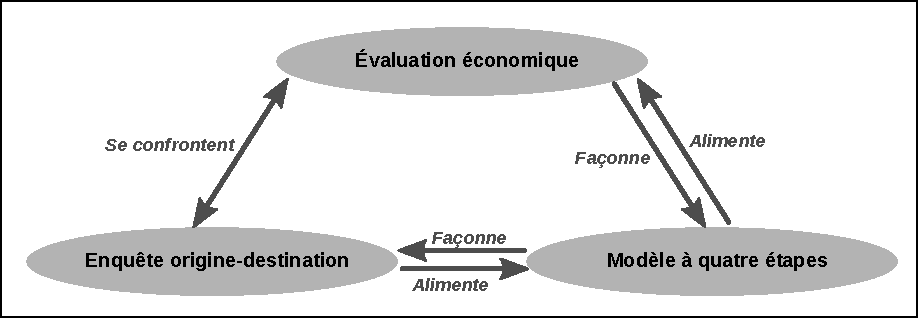
\includegraphics[width=12cm]{Interrelations.pdf}
\end{figure}

\end{frame}


% FRAME
\begin{frame}{Importation des instruments techniques}

\begin{itemize}
  \item Le Corps des Ponts et Chaussées et la \textbf{planification rationnelle}.
\end{itemize}

\begin{figure}
  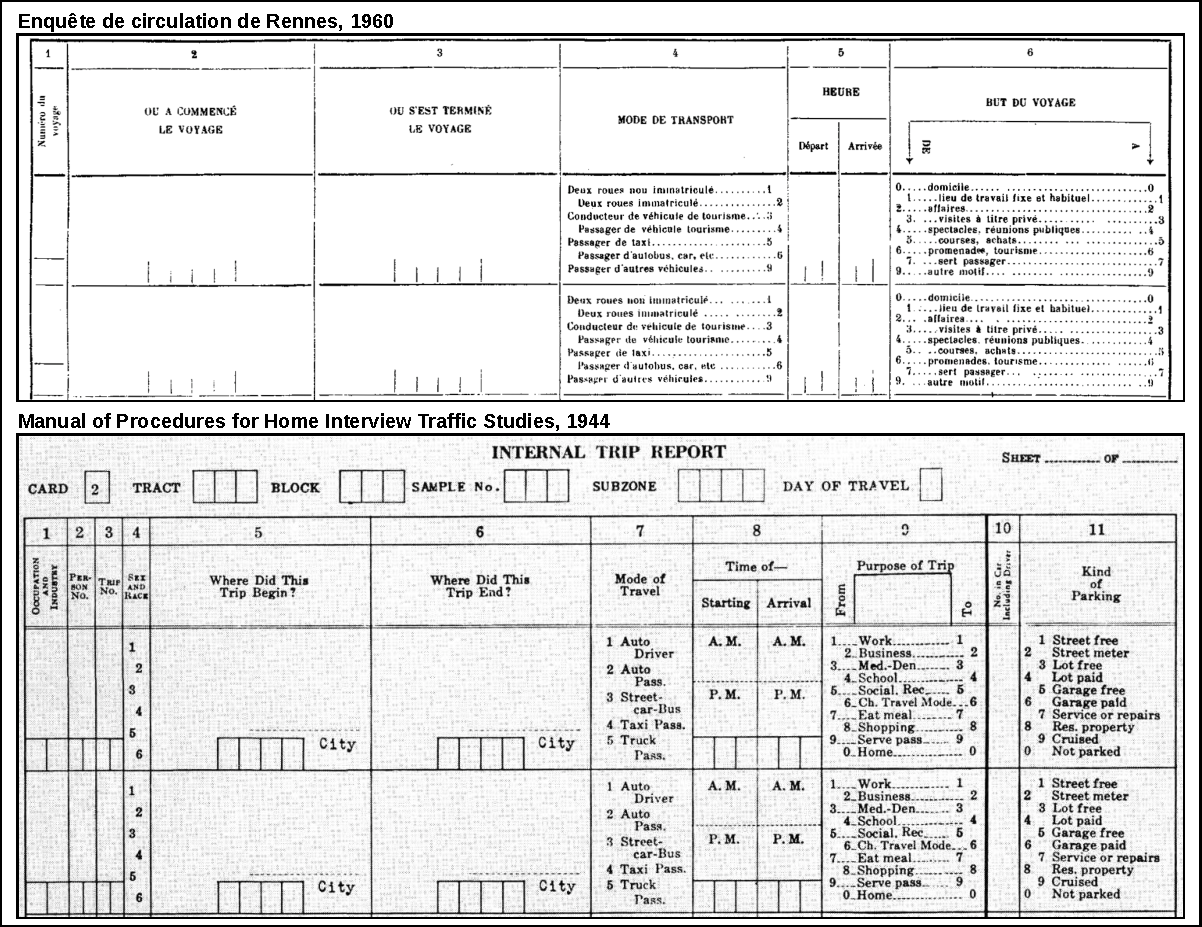
\includegraphics[width=9cm]{EMDRennes.pdf}
\end{figure}

\end{frame}


% FRAME
\begin{frame}{Typologie des instruments de mesure}

\begin{itemize}
  \item \textbf{Naissance de l'objet \textit{mobilité quotidienne}:} ingeniérie du trafic et sociologie urbaine
  \item \textbf{Constitution des instruments:} ingeniérie du traffic et socio-économie des transports
\end{itemize}

\begin{figure}
  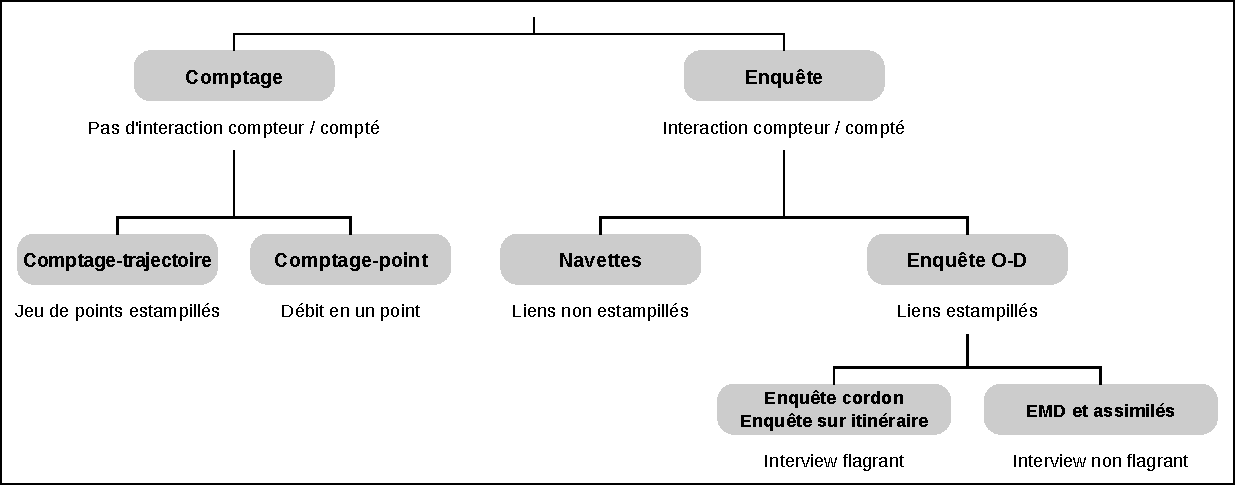
\includegraphics[width=12cm]{TypesEnquetes.pdf}
\end{figure}

\end{frame}






%%%%%% Là c'est à toi Julie !!!
% FRAME
\begin{frame}{Nouvelles sources de données}

Là c'est à toi Julie !!!

\begin{itemize}
  \item D'abord ça
  \item Et puis ça
  \item Et puis finalement ça
\end{itemize}

\end{frame}






% FRAME
\begin{frame}{Présentation de l'exercice}

\textbf{Deux espaces - Deux sources de données:}

\begin{enumerate}
  \item Mobilité quotidienne à New York d'après les données Citibike.
  \item Mobilité quotidienne à Marseille d'après les données Twitter.
\end{enumerate}

\textbf{Choisir un exercice et examiner les données disponibles:}

\begin{itemize}
  \item Données spécifiques (Citibike ou Twitter, fichier .csv)
  \item Navettes domicile-travail (fichier .csv)
  \item Fond de carte de l'espace d'étude (fichier .shp)
\end{itemize}

\textbf{Produit attendu:}

\begin{itemize}
  \item Présentation orale de 20 mn.
  \item Dossier écrit court et efficace: 4 pages, contenant graphique(s), carte(s), tableau(x). Publication de type \textit{Population et sociétés} \footnotesize <\url{http://www.ined.fr/fr/publications/population-et-societes}> \normalsize
\end{itemize}

\end{frame}



% FRAME
\begin{frame}{Questions, objets, mesures}

\textbf{Avant de mettre les mains dans les données}, il faut répondre aux questions suivantes:

\begin{enumerate}
  \item \textbf{Question(s):} à quelle(s) question(s) je cherche à répondre? 
  \item \textbf{Objet(s):} quel(s) objet(s) définir pour répondre à la question: communes, stations, individus, trajets, etc.
  \item \textbf{Mesure(s):} quelles mesures appliquer sur ces objets pour répondre à la question?
  \item \textbf{Chaîne de traitement:} quels traitements et quelle articulation entre les traitements pour passer des données des brutes à des mesures spécifiques répondant à la question?
\end{enumerate}

\end{frame}


% FRAME
\begin{frame}{Analyser des objets}

Pour déterminer les traitements à effectuer sur les objets et penser leur articulation, il faut:

\begin{itemize}
  \item Savoir identifier les objets et leurs propriétés. 
  \item Maîtriser l'emboîtement des objets et la création de propriétés dérivées.
\end{itemize}

\begin{figure}
  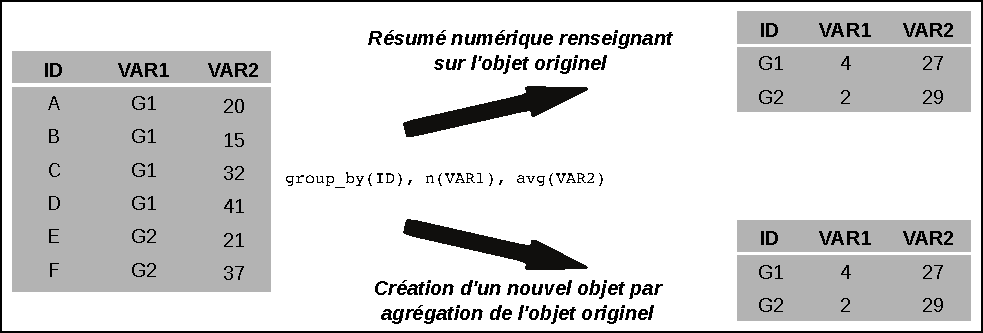
\includegraphics[width=12cm]{AnalyseObjets.pdf}
\end{figure}

\end{frame}


% FRAME
\begin{frame}{Analyser des relations}

Pour déterminer les traitements à effectuer sur les flux et penser leur articulation, il faut:

\begin{itemize}
  \item Comprendre les deux formats de stockage classiques. 
  \item Savoir quels sont les avantages respectifs de ces deux formats.
  \item Savoir passer d'un format à l'autre.
\end{itemize}

\begin{figure}
  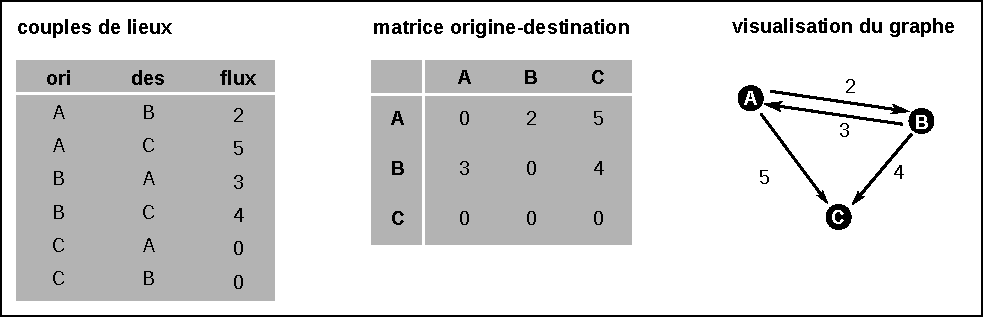
\includegraphics[width=12cm]{AnalyseRelations.pdf}
\end{figure}

\end{frame}

% FRAME BIBLIO 1
\begin{frame}{Bibliographie}

\textbf{Travaux sur et/ou avec les EMD:}

\footnotesize
\begin{itemize}
  \item Publications du CERTU (CEREMA): rapports techniques sur la constitution des EMD (p.ex. \textit{L'enquête ménages déplacements méthode standard}), rapports de synthèse à partir des EMD (p.ex. \textit{La mobilité urbaine en France}), travaux thématiques sur les EMD (p.ex. \textit{Et si les Français n'avaient plus seulement une voiture dans la tête?}).
  \item Banos A., Thévenin Th. (2005) \og Révéler les rythmes urbains par la carte animées \fg{}, \emph{Revue internationale de géomatique}, vol.15, nº1, pp.11.32.
  \item Commenges H. (2013) \textit{L'invention de la mobilité quotidienne}, Thèse de doctorat, Université Paris Diderot, Paris.
  \item Kaufmann V. (2008) \textit{Les paradoxes de la mobilité}, Presses polytechniques et universitaires romandes, Lausanne.
  \item Tabaka K. (2009) \textit{Vers une nouvelle socio-géographie de la mobilité quotidienne}, Thèse de doctorat, Université Joseph Fourier, Grenoble.
\end{itemize}

\normalsize
\end{frame}


% FRAME BIBLIO 2
\begin{frame}{Bibliographie (suite)}

\textbf{Mobilité quotidienne et planification des transports:}

\footnotesize
\begin{itemize}
  \item Dupuy G. (1975) Une technique de planification au service de l'automobile. Les modèles de trafic urbain, Ministère de l'équipement, Paris.
  \item Flonneau M., Guigueno V.(2009) \textit{De l'histoire des transports à l'histoire de la mobilité?}, Presses universitaires de Rennes, Rennes.
  \item Offner J.-M. (1993) \og Les ``effets structurants'' du transport: mythe politique, mystification scientifique \fg{}, \textit{L'Espace géographique}, vol.22, nº3, pp.233-242.
  \item Raux Ch., Andan O., Bonnel P. (1988) \textit{Les analyses des comportements de mobilité individuelle quotidienne: une synthèse bibliographique}, Laboratoire d'Economie des Transports, Lyon.
\end{itemize}

\normalsize
\end{frame}


% FRAME BIBLIO 3
\begin{frame}{Bibliographie (suite)}

\textbf{Mobilité et TIC - aspects performatifs:}

\footnotesize
\begin{itemize}
  \item Ascher F. (1995) \emph{Métapolis ou l’avenir des villes}, Paris, Odile jacob (Chapitre 2).
  \item Massot M.H. (1995) \emph{Transports et télécommunications}, Editions Paradigme.
  \item Mokhtarian P. (1990) "A tipology of relationships between telecommunications and transportation", \emph{Transportation Research A}, vol.24, nº3, pp.231-242.
  \item Rallet A. \emph{et al.} (2009) "Diffusion des TIC et mobilité : permanence et renouvellement des problématiques de recherche", \emph{Flux}, nº78, pp.7-16.
  \item Savy M. (1998) \og TIC et territoire: le paradoxe de localisation \fg{}, \textit{Cahiers Scientifiques du Transport}, vol.33, pp.129-146.
\end{itemize}

\normalsize
\end{frame}


% FRAME BIBLIO 4
\begin{frame}{Bibliographie (suite)}

\textbf{Mobilité et TIC - aspects descriptifs:}

\footnotesize
\begin{itemize}
  \item Austwick M.Z., O'Brien O., Strano E., Viana M. (2013) "The structure of spatial networks and communities in bicycle sharing systems", \textit{PLOS ONE}, vol.8, nº9.
  \item Fen-Chong J. (2012) \textit{Organisation spatio-temporelle des mobilités révélées par la téléphonie mobile en Île-de-France}, Thèse de doctorat, Université Paris 1.
  \item Ferreira N. \emph{et al.} (2013) "Visual exploration of big spatio-temporal urban data", \emph{Transactions on Visualization and Computer Graphics}, vol.19, nº12, pp.2149-2158.
  \item Goodchild M.F. (2007) "Citizens as voluntary sensors : spatial data infrastructure in the world of Web 2.0", \emph{International Journal of Spatial Data Infrastructure Research}, vol.2, pp.24–32.
  \item Joliveau T. (2011) "Le géoweb, un nouveau défi pour les bases de données géographiques", \emph{L'Espace géographique}, vol.40, nº2, pp.154–163.
\end{itemize}

\normalsize
\end{frame}





\end{document}
